\documentclass[11pt,a4paper]{article}

\usepackage[margin=2.5cm]{geometry}
\usepackage{xcolor}
\usepackage{graphicx}
\usepackage{fancyhdr}
\usepackage{titlesec}
\usepackage{enumitem}
\usepackage{listings}
\usepackage{hyperref}
\usepackage{parskip}
\usepackage{tabularx}
\usepackage{booktabs}

\definecolor{accent}{HTML}{0B78B8}    % darkened Omarchy accent, printable on white
\definecolor{codebg}{HTML}{F4F6FA}
\definecolor{coderule}{HTML}{C7D3E8}
\definecolor{mutedtext}{HTML}{5A6B85}

\titleformat{\section}{\Large\bfseries\color{accent}}{\thesection}{0.5em}{}
\titleformat{\subsection}{\large\bfseries\color{accent}}{\thesubsection}{0.5em}{}

\pagestyle{fancy}
\fancyhf{}
\renewcommand{\headrulewidth}{0.4pt}
\fancyhead[L]{\small\textcolor{mutedtext}{tsw-steam-bridge}}
\fancyhead[R]{\small\textcolor{mutedtext}{User Manual}}
\fancyfoot[C]{\small\thepage}

\lstdefinestyle{shell}{
    backgroundcolor=\color{codebg},
    basicstyle=\ttfamily\small,
    frame=single,
    rulecolor=\color{coderule},
    framerule=0.6pt,
    xleftmargin=0.5em,
    xrightmargin=0.5em,
    breaklines=true,
    columns=fullflexible,
}
\lstset{style=shell}

\hypersetup{
    colorlinks=true,
    linkcolor=accent,
    urlcolor=accent,
    citecolor=accent,
    pdftitle={tsw-steam-bridge User Manual},
    pdfauthor={tsw-steam-bridge},
}

\newcommand{\code}[1]{\texttt{#1}}

\title{\textcolor{accent}{\Huge tsw-steam-bridge}\\[0.3em]\Large User Manual}
\author{}
\date{\today}

\begin{document}

\maketitle
\thispagestyle{empty}

\vspace{1cm}
\noindent
A Zig bridge between Steam Input and Train Sim World: it reads real Steam
Input digital/analog actions and drives Train Sim World's cab controls
directly through its external HTTP API, instead of going through Steam
Input's keyboard/mouse emulation.

\vspace{0.5cm}
\noindent
\textbf{Why this exists:} keyboard emulation flattens two things Train Sim
World needs kept apart. Throttle and brake want continuous values, not
just ``tapped'' or ``held''. And safety controls like AWS (Automatic
Warning System) reset and DSD (Driver's Safety Device / vigilance) reset
are separate physical controls in the real cab that often end up sharing
or fighting over the same key in a simple keybind scheme. This bridge
keeps them independent by talking to Steam Input's real action API and to
Train Sim World's real control API, with nothing synthetic in between.

\newpage
\tableofcontents
\newpage

\section{Overview}

The project has three executables, built from the same source tree:

\begin{center}
\begin{tabularx}{\textwidth}{@{}l X@{}}
\toprule
\textbf{Executable} & \textbf{Purpose} \\
\midrule
\code{tsw-cli} & Pure Zig, no external dependencies. Talks to Train Sim
World's \code{-HTTPAPI} over plain HTTP. Use it to check the API is
reachable, explore a locomotive's control tree, and hand-test individual
values. \\[0.5em]
\code{steam-bridge} & The actual bridge process. Links against the
Steamworks SDK to read real Steam Input actions and writes their values
into Train Sim World via the same client code \code{tsw-cli} uses. \\[0.5em]
\code{tsw-gui} & A live dashboard shell built on Dear ImGui, themed from
your Omarchy colors and font, with dockable panels. \\
\bottomrule
\end{tabularx}
\end{center}

Control names are \textbf{not consistent across locomotives} --- not even
across versions of the same class --- so there is no single, universal
``AWS reset'' path in Train Sim World's API. Instead, each locomotive gets
its own small JSON \emph{profile} under \path{profiles/}, mapping a stable
set of logical control names (\code{throttle}, \code{aws\_reset},
\code{dsd\_reset}, \ldots) onto that particular locomotive's real node
paths. You build these up over time, one locomotive at a time, using
\code{tsw-cli discover}.

\section{Prerequisites}

\begin{itemize}[leftmargin=1.5em]
    \item \textbf{Zig 0.16.0 or newer.}
    \item \textbf{Train Sim World}, launched with the \code{-HTTPAPI}
    Steam launch option (see Section~\ref{sec:tsw-api}).
    \item \textbf{The Steamworks SDK}, vendored locally (see
    Section~\ref{sec:sdk}) --- needed to build \code{steam-bridge}.
    \item \textbf{A Steam client}, running and logged in, for
    \code{steam-bridge} and any Steam Input functionality.
\end{itemize}

\code{tsw-cli} needs none of the above except Zig itself, so it is the
easiest place to start.

\section{Enabling Train Sim World's external API}
\label{sec:tsw-api}

Train Sim World ships a real, officially-documented external control API
--- Dovetail's own \emph{External Interface API v1.5} document (written
for TSW6, and confirmed working exactly as described against a live TSW7
session while building this project). To enable it:

\begin{enumerate}[leftmargin=1.5em]
    \item In Steam, open Train Sim World's properties and add
    \code{-HTTPAPI} to the launch options.
    \item Launch the game once. This writes a file called
    \code{CommAPIKey.txt} under\\
    \path{Documents/My Games/TrainSimWorld<N>/Saved/Config/} (where
    \code{<N>} is the game's version number).
    \item If you're running Train Sim World through Proton, that path is
    inside the Proton prefix, typically under something like\\
    \path{~/.local/share/Steam/steamapps/compatdata/<appid>/pfx/} \\
    \path{drive_c/users/steamuser/My Documents/My Games/...}. \\
    The quickest way to find it is:
\begin{lstlisting}
find ~/.steam ~/.local/share/Steam -iname CommAPIKey.txt
\end{lstlisting}
\end{enumerate}

Every request to the API must include the contents of that file in a
\code{DTGCommKey} HTTP header --- the tools in this project handle that for
you once you point them at the file with \code{--key-file}.

The API listens on \code{http://localhost:31270} --- confirmed the same
port on a live TSW7 session, build 834; run \code{tsw-cli info} to confirm
it on your own install too (Section~\ref{sec:cli-info}).

\section{Vendoring the Steamworks SDK}
\label{sec:sdk}

\code{steam-bridge} needs Valve's Steamworks SDK, which is not
redistributable and must be downloaded yourself:

\begin{enumerate}[leftmargin=1.5em]
    \item Sign in with any Steam account at
    \url{https://partner.steamgames.com/downloads/list} and download
    \code{steamworks\_sdk.zip}.
    \item Extract it into the project so that
    \path{vendor/sdk/public/...} and
    \path{vendor/sdk/redistributable_bin/...} exist.
\end{enumerate}

\code{vendor/sdk/} is git-ignored --- it is a large, license-encumbered
redistributable, not part of the project's source. \code{zig build} will
still build \code{tsw-cli} and \code{tsw-gui} without it; it only skips
\code{steam-bridge}.

\subsection*{Why app id 480}

Steam Input's API needs to run as some recognized Steam application ---
\code{SteamAPI\_Init} needs a \code{steam\_appid.txt} file (or a
\code{SteamAppId} environment variable) naming one. For a personal,
unpublished tool like this, the standard approach used across the
community is Valve's public ``Spacewar'' test application, id \code{480}.
\code{steam-bridge} writes \code{steam\_appid.txt} containing \code{480}
automatically on first run if it is missing. If you ever publish this
project under your own Steam app id, replace that file's contents and
regenerate \path{manifest/game_actions_480.vdf} for your id.

\section{Building}

From the project root:

\begin{lstlisting}
zig build
\end{lstlisting}

This builds \code{tsw-cli} and \code{tsw-gui} unconditionally, and
\code{steam-bridge} if the Steamworks SDK has been vendored (Section
\ref{sec:sdk}). The GUI's own dependencies (zgui, zglfw, zopengl) are
fetched automatically the first time you build.

Binaries land in \path{zig-out/bin/}. You can also run them directly
through the build system, which forwards arguments after \code{--}:

\begin{lstlisting}
zig build run-cli    -- info --key-file /path/to/CommAPIKey.txt
zig build run-bridge -- --key-file /path/to/CommAPIKey.txt
zig build run-gui
\end{lstlisting}

\subsection*{A note if you're building this yourself on a similar system}

On some current Linux systems, Zig 0.16.0's own linker cannot yet handle
the \code{.sframe} unwind sections that current glibc/gcc toolchains emit
--- any libc-linked Zig binary fails to link with an error mentioning
\code{unhandled relocation type R\_X86\_64\_PC64 ... .sframe}. If you hit
this, it is a toolchain issue, not a problem with your setup specifically;
this project's own \path{build.zig} already works around it for
\code{steam-bridge} and \code{tsw-gui} by linking those two through the
system \code{cc}/\code{c++} instead of Zig's built-in linker.

\section{tsw-cli --- exploring and testing the API}
\label{sec:cli-info}

\code{tsw-cli} is the tool you reach for first: it talks to Train Sim
World directly over HTTP and does nothing with Steam Input at all.

\subsection{Checking the API is reachable}

\begin{lstlisting}
tsw-cli --key-file /path/to/CommAPIKey.txt info
\end{lstlisting}

A successful response confirms the port and prints the game's name and
build number, which is the fastest way to sanity-check that
\code{-HTTPAPI} took effect and that the port hasn't moved on your version
of the game.

\subsection{Listing controls}

\begin{lstlisting}
tsw-cli --key-file <key> list CurrentDrivableActor
\end{lstlisting}

Lists the child nodes and endpoints of whatever locomotive you are
currently driving --- this is how you discover what is actually
controllable on a given loco, since names vary by locomotive class.

\subsection{Reading and writing values}

\begin{lstlisting}
tsw-cli --key-file <key> get CurrentDrivableActor/Throttle_F.InputValue
tsw-cli --key-file <key> set CurrentDrivableActor/PanUp.InputValue 1
\end{lstlisting}

The writable endpoint on every interactive control --- lever, button, or
switch --- is always named \code{InputValue}, confirmed against DTG's own
documentation. \textbf{It only ever accepts a number, even for a control
that's conceptually a boolean:} sending \code{true}/\code{false} fails
with \code{\{"Result":"Error","Message":"Invalid Value (Not a Float)"\}}
--- use \code{1}/\code{0} instead. Use \code{set} carefully and only while
stationary until you know what a control actually does.

Every lever-style control also exposes real, documented functions for its
own metadata --- worth querying instead of guessing:

\begin{lstlisting}
tsw-cli --key-file <key> get CurrentDrivableActor/Reverser.Function.GetNotchCount
tsw-cli --key-file <key> get CurrentDrivableActor/Reverser.Function.GetMinimumInputValue
tsw-cli --key-file <key> get CurrentDrivableActor/Reverser.Function.GetMaximumInputValue
\end{lstlisting}

Note that \code{Function.} is part of the endpoint name itself, not a
separator you add. \textbf{Don't assume every lever's range is 0..1} ---
confirmed live across two different locomotives that this varies: see the
worked example in Section~\ref{sec:worked-examples}.

\subsection{Building a locomotive profile}
\label{sec:discover}

\begin{lstlisting}
tsw-cli --key-file <key> discover
\end{lstlisting}

Walks the current locomotive's writable controls and writes a skeleton
profile to \path{profiles/<ObjectClass>.json}, where \code{<ObjectClass>}
is that locomotive's internal class name. The skeleton lists every
candidate writable control under its raw node name; you then:

\begin{enumerate}[leftmargin=1.5em]
    \item Test each candidate path with \code{tsw-cli set <path> 1} (or
    \code{0}, or a float) while parked, and observe what happens in the
    cab.
    \item Rename the JSON key to the matching logical name the bridge
    expects. The full, current list --- covering core cab controls plus
    British (AWS/DSD/TPWS/DRA), German (SIFA/PZB/LZB) and ETCS actions
    --- is kept in \path{profiles/README.md} rather than duplicated here,
    since it grows as the bridge's control vocabulary does.
    \item Fix \code{"kind"} to \code{"float"} for anything that isn't a
    plain on/off control, and add a \code{"range"} override (Section
    \ref{sec:worked-examples}) if this control's \code{GetMinimumInputValue}/
    \code{GetMaximumInputValue} isn't 0..1.
    \item Delete entries you don't care about mapping --- an incomplete
    profile is fine; the bridge simply skips logical controls that
    aren't mapped for the current locomotive.
\end{enumerate}

\subsection{Worked example: two real locomotive profiles}
\label{sec:worked-examples}

Two locomotive profiles ship with the project already, both built
entirely from live TSW7 sessions using the workflow above, not guessed:

\begin{itemize}[leftmargin=1.5em]
    \item \path{profiles/RVM_AWL_NT_Class333_DMSO_B_C.json} --- British
    Rail Class 333 (DMSO), a single-cab EMU with one combined
    power/brake handle. Its \code{CombinedPowerBrakeHandle.InputValue}
    runs 0..1 (9 notches, confirmed via
    \code{Function.GetNotchCount}/\code{GetMaximumInputValue}), and its
    \code{Reverser} is a 4-notch lever, also 0..1. No PZB/SIFA/LZB or
    ETCS mapped --- it's a British unit that doesn't carry them.
    \item \path{profiles/RVM_AWL_NT_Class331_DMS_C.json} --- British Rail
    Class 331 (DMS), also a combined-handle EMU, but its
    \code{PowerBrakeController.InputValue} genuinely reports \textbf{-1..1}
    rather than 0..1 (5 notches) --- confirmed live by querying that
    control's own \code{Function.GetMinimumInputValue}/
    \code{GetMaximumInputValue}, then moving it and watching the value
    snap to notch positions. This locomotive also needs its
    \code{MasterKey} switched on and its \code{Reverser} moved out of
    neutral before \code{PowerBrakeController} has any effect at all ---
    worth checking first on any unfamiliar locomotive if power/brake
    seems unresponsive.
\end{itemize}

Discovering the second locomotive's real range is exactly why the profile
format has a \code{"range"} override field (Section
\ref{sec:profile-format}) --- assuming every lever shares the first
locomotive's 0..1 range turned out to be wrong the moment a second one
was tested. Always check \code{GetMinimumInputValue}/
\code{GetMaximumInputValue} on a new locomotive rather than assuming.

\section{steam-bridge --- running the live bridge}
\label{sec:steam-bridge}

Once you have a locomotive profile and the Steamworks SDK vendored:

\begin{lstlisting}
zig build run-bridge
\end{lstlisting}

You don't need \code{--key-file} by hand: if it's omitted,
\code{steam-bridge} (and \code{tsw-gui}) search for \code{CommAPIKey.txt}
themselves across every Steam library and Proton prefix they can find
(Section~\ref{sec:tsw-api}), picking the most recently modified match if
more than one Train Sim World version is installed. Pass \code{--key-file}
explicitly if you need to override that.

On startup, \code{steam-bridge} initializes the Steamworks API, activates
its own \code{Driving} Steam Input action set (defined in
\path{manifest/game_actions_480.vdf}, entirely separate from Train Sim
World's own Steam Input configuration), and begins polling. Every tick it:

\begin{enumerate}[leftmargin=1.5em]
    \item Reads the current locomotive's class from Train Sim World and
    loads the matching profile from \path{profiles/}.
    \item Polls each logical Steam Input action --- \code{throttle},
    \code{brake} and \code{combined\_power\_brake} as analog axes or
    stepped detents depending on the active profile's setting for that
    lever, the rest as digital buttons.
    \item For anything that changed and has a mapping in the active
    profile, sends the new value to Train Sim World via \code{PATCH
    /set/...}.
\end{enumerate}

\subsection*{Notched vs.\ notchless levers}

Real locomotives have both kinds of throttle/brake handle, and holding an
auto-centering analog stick at one precise deflection to maintain line
speed for an hour is uncomfortable at best. So each of \code{throttle},
\code{brake} and \code{combined\_power\_brake} can instead be driven by a
pair of up/down detent actions (\code{throttle\_up}/\code{throttle\_down},
etc.) that \code{steam-bridge} accumulates into an absolute position
itself --- snapped to a fixed number of notches, or stepped by a tunable
amount for a notchless lever. This is controlled per-lever by that
control's \code{"mode"} field in its locomotive profile
(\code{"absolute"}, \code{"notched"} with a \code{"notches"} count, or
\code{"notchless"} with a \code{"step\_size"}); see
\path{profiles/README.md} for the full field reference. The default step
size for notchless levers can be overridden globally with
\code{steam-bridge --step-size <value>}.

A detent-based binding pairs naturally with Steam Input's trackpad
``Scroll Wheel'' mode set to circular swipe, which turns a flat trackpad
into a haptic rotary encoder --- but any pair of buttons or paddles works
just as well.

\textbf{Current status:} Steam's own API confirms successful
initialization against a real, running Steam client, but activating the
custom action manifest is not yet reliably working end-to-end --- this is
the active area of development. See the project README's ``Known gaps''
section for the latest status. Note that \code{tsw-gui} runs this exact
same bridge internally (Section~\ref{sec:tsw-gui}); running both at once
against the same controller and profile isn't useful and will have them
race each other's \code{/set} calls, so pick one or the other.

\section{Binding physical controls in Steam}
\label{sec:steam-binding}

Steam Input has no idea what a \code{combined\_power\_brake} action
should map to on your specific controller until you tell it, and that
binding lives entirely inside Steam's own UI --- this project never reads
or writes controller bindings itself. It only declares what actions exist
(\path{manifest/game_actions_480.vdf}) and polls whatever Steam reports
for them once you've bound them.

Because this is a personal, unpublished tool rather than something
published under its own Steam app id, it identifies itself to Steam as
Valve's public ``Spacewar'' test application, id \code{480} (Section
\ref{sec:sdk}). That has one very concrete consequence for you: \textbf{the
game you configure controller bindings for inside Steam is called
``Spacewar,'' not ``Train Sim World.''}

\begin{enumerate}[leftmargin=1.5em]
    \item \textbf{Install Spacewar once}, if you haven't already --- it's
    free. From the Steam client, open the Store and search for
    ``Spacewar,'' or navigate directly to \url{steam://install/480} and
    install it. This doesn't launch a real game; it's a lightweight test
    application Valve ships specifically so indie developers can exercise
    Steam Input without owning a published app id.
    \item \textbf{Launch \code{steam-bridge} or \code{tsw-gui}} (either
    one). On startup it calls \code{SteamAPI\_Init} claiming app id 480,
    so Steam now treats this project's own process as if it were Spacewar
    currently running.
    \item \textbf{Open Steam's controller configurator for Spacewar.} The
    most reliable path is Big Picture Mode: Steam
    $\rightarrow$ View $\rightarrow$ Big Picture Mode $\rightarrow$
    Library $\rightarrow$ find Spacewar (it will show as ``Running'')
    $\rightarrow$ the controller/gear icon $\rightarrow$ Controller
    Options $\rightarrow$ Configure. Desktop Steam sometimes offers the
    same screen via the controller icon in the top-right of the client
    while \code{steam-bridge}/\code{tsw-gui} is running, but Big Picture
    Mode is the version that reliably surfaces a game's custom action
    manifest.
    \item \textbf{Bind every action.} Steam shows the \code{Driving}
    action set from \path{manifest/game_actions_480.vdf} and every action
    it declares --- \code{combined\_power\_brake}, \code{throttle},
    \code{brake}, \code{reverser}, all four \code{\_up}/\code{\_down}
    notch-stepping pairs, and every digital control (\code{horn},
    \code{aws\_reset}, \code{master\_key\_toggle}, \ldots). Bind analog
    sticks/triggers to the three levers' absolute axes, any button/paddle
    to the digital controls, and --- for a notched lever's tactile
    ``rotary encoder'' feel --- a trackpad set to ``Scroll Wheel''
    (circular) mode bound to that lever's \code{\_up}/\code{\_down} pair
    (Section~\ref{sec:steam-bridge}).
    \item \textbf{Save the configuration.} Steam applies it immediately;
    \code{steam-bridge}/\code{tsw-gui} reflects your input the moment you
    move or press a bound control, visible live in \code{tsw-gui}'s
    panels (Section~\ref{sec:tsw-gui}).
\end{enumerate}

\textbf{Current status:} as noted at the end of
Section~\ref{sec:steam-bridge}, this project's own call to activate its
custom action manifest is not yet confirmed reliably working end-to-end,
independently of everything above --- Steam Input's own initialization
and the app-id-480 identification both work, but the custom \code{Driving}
action set may not appear or activate correctly for you yet. If bindings
made this way don't seem to reach \code{steam-bridge}/\code{tsw-gui}, that
is the known gap tracked in the project README, not a step you've missed.

\section{tsw-gui --- the live dashboard}
\label{sec:tsw-gui}

\code{tsw-gui} is a windowed dashboard with dockable panels, built on Dear
ImGui, that runs the exact same live bridge as \code{steam-bridge}
internally --- it isn't a separate visualization of a running
\code{steam-bridge}, it drives Steam Input and Train Sim World directly
itself, once per rendered frame. Just run it:

\begin{lstlisting}
./zig-out/bin/tsw-gui
\end{lstlisting}

No arguments are required for a first look: it finds your key file the
same way \code{steam-bridge} does (Section~\ref{sec:tsw-api}) and falls
back to a clearly-labeled preview mode if nothing is found or Steam isn't
running, rather than failing to start. Its font is bundled into the
binary (JetBrains Mono, SIL OFL~1.1), so it looks right with no setup on
any platform.

The panels are generated from the same control list \code{steam-bridge}
uses (\path{src/controls.zig}), so the dashboard always reflects the
actual current set of controls, not a fixed example:

\begin{itemize}[leftmargin=1.5em]
    \item \textbf{Status} --- Steam Input/controller connection, active
    locomotive, and whether a profile was found for it.
    \item \textbf{Power \& Brake} --- a live progress bar and mode
    (absolute / notched / notchless) for each of the three levers.
    \item One tabbed panel per remaining category --- Core Cab, British
    Safety, German Safety, ETCS --- listing every control in that
    category, colored dim if unmapped for the current locomotive, normal
    if mapped, and in the theme's accent color while actively pressed.
\end{itemize}

Figure~\ref{fig:screenshot} shows this layout: the Status and Power \&
Brake panels docked on the left, and the ETCS tab selected among the
category panels on the right, themed from the Coaster theme's palette and
set in the bundled JetBrains Mono font.

\begin{figure}[h]
    \centering
    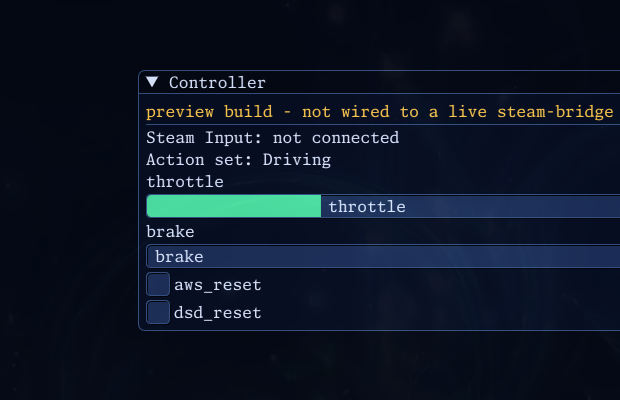
\includegraphics[width=\textwidth]{images/tsw-gui-screenshot.png}
    \caption{tsw-gui's default docked layout: Status and Power \& Brake
    on the left, tabbed category panels on the right.}
    \label{fig:screenshot}
\end{figure}

Panels can be dragged by their title bar to rearrange or dock them
differently. The first time you run \code{tsw-gui} (before an
\path{imgui.ini} exists in the working directory), it builds the layout
shown above automatically; from then on, Dear ImGui saves whatever
arrangement you leave it in to \path{imgui.ini} and restores it on
every subsequent launch.

On Linux, colors are additionally read live from your active Omarchy
theme's \path{colors.toml} at startup rather than hardcoded, so the panel
follows whichever theme is active system-wide; elsewhere (or on Linux
without Omarchy) it falls back to the same colors shown here. Pass
\code{--theme-file}/\code{--font-file} to override either explicitly, or
on Linux use \code{scripts/run-gui.sh} to match your current Omarchy font
specifically:

\begin{lstlisting}
./scripts/run-gui.sh
\end{lstlisting}

\textbf{Current status:} see the note at the end of
Section~\ref{sec:steam-bridge} --- Steam Input manifest activation isn't
reliably working end-to-end yet, so the live values shown will generally
read as inactive/zero until that's resolved. Run only one of
\code{tsw-gui} or \code{steam-bridge} at a time against the same
controller and profile.

\section{Troubleshooting}

\begin{center}
\begin{tabularx}{\textwidth}{@{}l X@{}}
\toprule
\textbf{Symptom} & \textbf{Likely cause / fix} \\
\midrule
\code{tsw-cli info} fails to connect &
Check \code{-HTTPAPI} is actually in Train Sim World's launch options and
the game has been launched at least once since adding it. Confirm the key
file path. Try the base URL override if your game version uses a
different port. \\[0.6em]
Steam Input fails with \code{NoSteamClient} &
Steam isn't running, or isn't fully started yet. Make sure Steam is open
and you are logged in before starting \code{steam-bridge}. \\[0.6em]
\code{zig build} skips \code{steam-bridge} &
The Steamworks SDK hasn't been vendored under \path{vendor/sdk/} --- see
Section~\ref{sec:sdk}. \\[0.6em]
A control does nothing when set &
Not every node listed by \code{discover} is meaningful --- some are
read-only telemetry mirrors or apply only to specific train sub-systems.
Cross-check against what changes in the cab. \\[0.6em]
\code{tsw-gui} shows the built-in font instead of my font &
Launch it via \path{scripts/run-gui.sh}, or pass \code{--font-file}
yourself with a real \code{.ttf}/\code{.otf} path. \\
\bottomrule
\end{tabularx}
\end{center}

\section{Reference: profile file format}
\label{sec:profile-format}

Profiles live at \path{profiles/<ObjectClass>.json}:

\begin{lstlisting}
{
  "objectClass": "RVM_AWL_NT_Class331_DMS_C",
  "displayName": "British Rail Class 331 (DMS)",
  "controls": {
    "combined_power_brake": {
      "path": "CurrentDrivableActor/PowerBrakeController.InputValue",
      "kind": "float",
      "mode": "notched",
      "notches": 5,
      "range": { "min": -1, "max": 1 }
    },
    "reverser": {
      "path": "CurrentDrivableActor/Reverser.InputValue",
      "kind": "float",
      "mode": "notched",
      "notches": 3
    },
    "aws_reset": { "path": "CurrentDrivableActor/AWS_Reset.InputValue", "kind": "bool" }
  }
}
\end{lstlisting}

(a real, verified entry from \path{profiles/RVM_AWL_NT_Class331_DMS_C.json}
--- see the worked example in Section~\ref{sec:worked-examples}.)

\begin{itemize}[leftmargin=1.5em]
    \item \code{path} --- the full API path, always ending in
    \code{.InputValue}.
    \item \code{kind} --- \code{"bool"} or \code{"float"}; controls how
    the bridge formats the value it sends to \code{PATCH /set/...}. TSW
    itself only ever accepts a number on the wire (\code{1}/\code{0} for
    a bool), regardless of this setting --- \code{kind} only affects how
    the bridge reads Steam Input's own digital/analog action data for
    this control.
    \item \code{mode}, \code{notches}, \code{step\_size} --- only apply to
    the three lever controls (\code{throttle}, \code{brake},
    \code{combined\_power\_brake}, or a locomotive's own name for the
    equivalent, like \code{reverser}); see Section~\ref{sec:steam-bridge}
    and \path{profiles/README.md} for the full mode reference.
    \item \code{range} --- optional \code{\{"min": ..., "max": ...\}}
    override for a lever's \code{InputValue} bounds. Defaults to 0..1
    (every lever's compiled-in default in \path{src/controls.zig}) when
    omitted. \textbf{Always check, never assume:} confirmed live that
    this genuinely varies by locomotive --- see Section
    \ref{sec:worked-examples}.
\end{itemize}

A logical control with no entry is simply never sent for that locomotive.

\end{document}
